% Options for packages loaded elsewhere
\PassOptionsToPackage{unicode}{hyperref}
\PassOptionsToPackage{hyphens}{url}
\PassOptionsToPackage{dvipsnames,svgnames,x11names}{xcolor}
%
\documentclass[
]{article}

\usepackage{amsmath,amssymb}
\usepackage{iftex}
\ifPDFTeX
  \usepackage[T1]{fontenc}
  \usepackage[utf8]{inputenc}
  \usepackage{textcomp} % provide euro and other symbols
\else % if luatex or xetex
  \usepackage{unicode-math}
  \defaultfontfeatures{Scale=MatchLowercase}
  \defaultfontfeatures[\rmfamily]{Ligatures=TeX,Scale=1}
\fi
\usepackage{lmodern}
\ifPDFTeX\else  
    % xetex/luatex font selection
\fi
% Use upquote if available, for straight quotes in verbatim environments
\IfFileExists{upquote.sty}{\usepackage{upquote}}{}
\IfFileExists{microtype.sty}{% use microtype if available
  \usepackage[]{microtype}
  \UseMicrotypeSet[protrusion]{basicmath} % disable protrusion for tt fonts
}{}
\makeatletter
\@ifundefined{KOMAClassName}{% if non-KOMA class
  \IfFileExists{parskip.sty}{%
    \usepackage{parskip}
  }{% else
    \setlength{\parindent}{0pt}
    \setlength{\parskip}{6pt plus 2pt minus 1pt}}
}{% if KOMA class
  \KOMAoptions{parskip=half}}
\makeatother
\usepackage{xcolor}
\setlength{\emergencystretch}{3em} % prevent overfull lines
\setcounter{secnumdepth}{-\maxdimen} % remove section numbering
% Make \paragraph and \subparagraph free-standing
\makeatletter
\ifx\paragraph\undefined\else
  \let\oldparagraph\paragraph
  \renewcommand{\paragraph}{
    \@ifstar
      \xxxParagraphStar
      \xxxParagraphNoStar
  }
  \newcommand{\xxxParagraphStar}[1]{\oldparagraph*{#1}\mbox{}}
  \newcommand{\xxxParagraphNoStar}[1]{\oldparagraph{#1}\mbox{}}
\fi
\ifx\subparagraph\undefined\else
  \let\oldsubparagraph\subparagraph
  \renewcommand{\subparagraph}{
    \@ifstar
      \xxxSubParagraphStar
      \xxxSubParagraphNoStar
  }
  \newcommand{\xxxSubParagraphStar}[1]{\oldsubparagraph*{#1}\mbox{}}
  \newcommand{\xxxSubParagraphNoStar}[1]{\oldsubparagraph{#1}\mbox{}}
\fi
\makeatother
\usepackage{color}
\usepackage{fancyvrb}
\newcommand{\VerbBar}{|}
\newcommand{\VERB}{\Verb[commandchars=\\\{\}]}
\DefineVerbatimEnvironment{Highlighting}{Verbatim}{commandchars=\\\{\}}
% Add ',fontsize=\small' for more characters per line
\usepackage{framed}
\definecolor{shadecolor}{RGB}{241,243,245}
\newenvironment{Shaded}{\begin{snugshade}}{\end{snugshade}}
\newcommand{\AlertTok}[1]{\textcolor[rgb]{0.68,0.00,0.00}{#1}}
\newcommand{\AnnotationTok}[1]{\textcolor[rgb]{0.37,0.37,0.37}{#1}}
\newcommand{\AttributeTok}[1]{\textcolor[rgb]{0.40,0.45,0.13}{#1}}
\newcommand{\BaseNTok}[1]{\textcolor[rgb]{0.68,0.00,0.00}{#1}}
\newcommand{\BuiltInTok}[1]{\textcolor[rgb]{0.00,0.23,0.31}{#1}}
\newcommand{\CharTok}[1]{\textcolor[rgb]{0.13,0.47,0.30}{#1}}
\newcommand{\CommentTok}[1]{\textcolor[rgb]{0.37,0.37,0.37}{#1}}
\newcommand{\CommentVarTok}[1]{\textcolor[rgb]{0.37,0.37,0.37}{\textit{#1}}}
\newcommand{\ConstantTok}[1]{\textcolor[rgb]{0.56,0.35,0.01}{#1}}
\newcommand{\ControlFlowTok}[1]{\textcolor[rgb]{0.00,0.23,0.31}{\textbf{#1}}}
\newcommand{\DataTypeTok}[1]{\textcolor[rgb]{0.68,0.00,0.00}{#1}}
\newcommand{\DecValTok}[1]{\textcolor[rgb]{0.68,0.00,0.00}{#1}}
\newcommand{\DocumentationTok}[1]{\textcolor[rgb]{0.37,0.37,0.37}{\textit{#1}}}
\newcommand{\ErrorTok}[1]{\textcolor[rgb]{0.68,0.00,0.00}{#1}}
\newcommand{\ExtensionTok}[1]{\textcolor[rgb]{0.00,0.23,0.31}{#1}}
\newcommand{\FloatTok}[1]{\textcolor[rgb]{0.68,0.00,0.00}{#1}}
\newcommand{\FunctionTok}[1]{\textcolor[rgb]{0.28,0.35,0.67}{#1}}
\newcommand{\ImportTok}[1]{\textcolor[rgb]{0.00,0.46,0.62}{#1}}
\newcommand{\InformationTok}[1]{\textcolor[rgb]{0.37,0.37,0.37}{#1}}
\newcommand{\KeywordTok}[1]{\textcolor[rgb]{0.00,0.23,0.31}{\textbf{#1}}}
\newcommand{\NormalTok}[1]{\textcolor[rgb]{0.00,0.23,0.31}{#1}}
\newcommand{\OperatorTok}[1]{\textcolor[rgb]{0.37,0.37,0.37}{#1}}
\newcommand{\OtherTok}[1]{\textcolor[rgb]{0.00,0.23,0.31}{#1}}
\newcommand{\PreprocessorTok}[1]{\textcolor[rgb]{0.68,0.00,0.00}{#1}}
\newcommand{\RegionMarkerTok}[1]{\textcolor[rgb]{0.00,0.23,0.31}{#1}}
\newcommand{\SpecialCharTok}[1]{\textcolor[rgb]{0.37,0.37,0.37}{#1}}
\newcommand{\SpecialStringTok}[1]{\textcolor[rgb]{0.13,0.47,0.30}{#1}}
\newcommand{\StringTok}[1]{\textcolor[rgb]{0.13,0.47,0.30}{#1}}
\newcommand{\VariableTok}[1]{\textcolor[rgb]{0.07,0.07,0.07}{#1}}
\newcommand{\VerbatimStringTok}[1]{\textcolor[rgb]{0.13,0.47,0.30}{#1}}
\newcommand{\WarningTok}[1]{\textcolor[rgb]{0.37,0.37,0.37}{\textit{#1}}}

\providecommand{\tightlist}{%
  \setlength{\itemsep}{0pt}\setlength{\parskip}{0pt}}\usepackage{longtable,booktabs,array}
\usepackage{calc} % for calculating minipage widths
% Correct order of tables after \paragraph or \subparagraph
\usepackage{etoolbox}
\makeatletter
\patchcmd\longtable{\par}{\if@noskipsec\mbox{}\fi\par}{}{}
\makeatother
% Allow footnotes in longtable head/foot
\IfFileExists{footnotehyper.sty}{\usepackage{footnotehyper}}{\usepackage{footnote}}
\makesavenoteenv{longtable}
\usepackage{graphicx}
\makeatletter
\def\maxwidth{\ifdim\Gin@nat@width>\linewidth\linewidth\else\Gin@nat@width\fi}
\def\maxheight{\ifdim\Gin@nat@height>\textheight\textheight\else\Gin@nat@height\fi}
\makeatother
% Scale images if necessary, so that they will not overflow the page
% margins by default, and it is still possible to overwrite the defaults
% using explicit options in \includegraphics[width, height, ...]{}
\setkeys{Gin}{width=\maxwidth,height=\maxheight,keepaspectratio}
% Set default figure placement to htbp
\makeatletter
\def\fps@figure{htbp}
\makeatother

\makeatletter
\@ifpackageloaded{caption}{}{\usepackage{caption}}
\AtBeginDocument{%
\ifdefined\contentsname
  \renewcommand*\contentsname{Table of contents}
\else
  \newcommand\contentsname{Table of contents}
\fi
\ifdefined\listfigurename
  \renewcommand*\listfigurename{List of Figures}
\else
  \newcommand\listfigurename{List of Figures}
\fi
\ifdefined\listtablename
  \renewcommand*\listtablename{List of Tables}
\else
  \newcommand\listtablename{List of Tables}
\fi
\ifdefined\figurename
  \renewcommand*\figurename{Figure}
\else
  \newcommand\figurename{Figure}
\fi
\ifdefined\tablename
  \renewcommand*\tablename{Table}
\else
  \newcommand\tablename{Table}
\fi
}
\@ifpackageloaded{float}{}{\usepackage{float}}
\floatstyle{ruled}
\@ifundefined{c@chapter}{\newfloat{codelisting}{h}{lop}}{\newfloat{codelisting}{h}{lop}[chapter]}
\floatname{codelisting}{Listing}
\newcommand*\listoflistings{\listof{codelisting}{List of Listings}}
\makeatother
\makeatletter
\makeatother
\makeatletter
\@ifpackageloaded{caption}{}{\usepackage{caption}}
\@ifpackageloaded{subcaption}{}{\usepackage{subcaption}}
\makeatother

\usepackage{hyphenat}
\usepackage{ifthen}
\usepackage{calc}
\usepackage{calculator}



\usepackage{graphicx}
\usepackage{geometry}
\usepackage{afterpage}
\usepackage{tikz}
\usetikzlibrary{calc}
\usetikzlibrary{fadings}
\usepackage[pagecolor=none]{pagecolor}


% Set the titlepage font families







% Set the coverpage font families


\ifLuaTeX
  \usepackage{selnolig}  % disable illegal ligatures
\fi
\usepackage{bookmark}

\IfFileExists{xurl.sty}{\usepackage{xurl}}{} % add URL line breaks if available
\urlstyle{same} % disable monospaced font for URLs
\hypersetup{
  colorlinks=true,
  linkcolor={blue},
  filecolor={Maroon},
  citecolor={Blue},
  urlcolor={Blue},
  pdfcreator={LaTeX via pandoc}}


\author{}
\date{}

\begin{document}
%%%%% begin titlepage extension code


\begin{titlepage}

%%% TITLE PAGE START

% Set up alignment commands
%Page
\newcommand{\titlepagepagealign}{
\ifthenelse{\equal{left}{right}}{\raggedleft}{}
\ifthenelse{\equal{left}{center}}{\centering}{}
\ifthenelse{\equal{left}{left}}{\raggedright}{}
}


\newcommand{\titleandsubtitle}{
% Title and subtitle
}
\newcommand{\titlepagetitleblock}{
\titleandsubtitle
}

\newcommand{\authorstyle}[1]{{#1}}

\newcommand{\affiliationstyle}[1]{{#1}}

\newcommand{\titlepageauthorblock}{
{\authorstyle{}}}

\newcommand{\titlepageaffiliationblock}{
\hangindent=1em
\hangafter=1
{\affiliationstyle{


\vspace{1\baselineskip} 
}}
}
\newcommand{\headerstyled}{%
{}
}
\newcommand{\footerstyled}{%
{}
}
\newcommand{\datestyled}{%
{}
}


\newcommand{\titlepageheaderblock}{\headerstyled}

\newcommand{\titlepagefooterblock}{
\footerstyled
}

\newcommand{\titlepagedateblock}{
\datestyled
}

%set up blocks so user can specify order
\newcommand{\titleblock}{}

\newcommand{\authorblock}{}

\newcommand{\affiliationblock}{}

\newcommand{\logoblock}{}

\newcommand{\footerblock}{}

\newcommand{\dateblock}{}

\newcommand{\headerblock}{}

\thispagestyle{empty} % no page numbers on titlepages


\newlength{\minipagewidth}
\setlength{\minipagewidth}{\textwidth}
\raggedright % single minipage
% [position of box][box height][inner position]{width}
% [s] means stretch out vertically; assuming there is a vfill
\begin{minipage}[b][\textheight][s]{\minipagewidth}
\titlepagepagealign
\headerblock

\titleblock

\authorblock

\affiliationblock

\vfill

\logoblock

\footerblock
\par

\end{minipage}\ifthenelse{\equal{}{right} \OR \equal{}{leftright} }{
\hspace{\B}
\vrulecode}{}
\clearpage
%%% TITLE PAGE END
\end{titlepage}
\setcounter{page}{1}

%%%%% end titlepage extension code


\section{Defining the regions for the operating
model}\label{defining-the-regions-for-the-operating-model}

Here we define the different regions to be used in the operating model,
based on the areas that were defined in the industry working groups. The
operating model is intended to encompass the Western Central Atlantic
dolphin population and include international waters
(\href{https://www.fao.org/fishery/en/area/search}{FAO areas 21 and 31})
which are thought to be connected with the stock that is exploited by
U.S. fisheries.

We use the U.S. exclusive economic zone (EEZ) to differentiate between
national and international waters. Note that some U.S. commercial
activity occurs in high seas waters and we will account for those
catches in the summaries.

\subsection{Data download for the U.S.
EEZ}\label{data-download-for-the-u.s.-eez}

We download the U.S. Atlantic EEZ from
\href{https://www.marineregions.org/gazetteer.php?p=details&id=8456}{Marineregions.org}.

\begin{Shaded}
\begin{Highlighting}[]
\CommentTok{\# clear workspace and load the libraries}
\FunctionTok{library}\NormalTok{(sf)}
\end{Highlighting}
\end{Shaded}

\begin{verbatim}
Warning: package 'sf' was built under R version 4.5.1
\end{verbatim}

\begin{verbatim}
Linking to GEOS 3.13.1, GDAL 3.11.0, PROJ 9.6.0; sf_use_s2() is TRUE
\end{verbatim}

\begin{Shaded}
\begin{Highlighting}[]
\FunctionTok{library}\NormalTok{(maps)}

\FunctionTok{rm}\NormalTok{(}\AttributeTok{list =} \FunctionTok{ls}\NormalTok{())}

\CommentTok{\# read in the shapefile downloaded from Marineregions.org}
\NormalTok{shp\_data }\OtherTok{\textless{}{-}} \FunctionTok{st\_read}\NormalTok{(}\StringTok{"data/eez/eez.shp"}\NormalTok{)}
\end{Highlighting}
\end{Shaded}

\begin{verbatim}
Reading layer `eez' from data source 
  `C:\Users\mandy.karnauskas\Desktop\SEFSC-dolphin-analyses\data\eez\eez.shp' 
  using driver `ESRI Shapefile'
Simple feature collection with 1 feature and 31 fields
Geometry type: MULTIPOLYGON
Dimension:     XY
Bounding box:  xmin: -129.2348 ymin: 23.83333 xmax: -65.69972 ymax: 49.00226
Geodetic CRS:  WGS 84
\end{verbatim}

\begin{Shaded}
\begin{Highlighting}[]
\NormalTok{coords }\OtherTok{\textless{}{-}} \FunctionTok{st\_coordinates}\NormalTok{(shp\_data)}
\NormalTok{co }\OtherTok{\textless{}{-}} \FunctionTok{as.data.frame}\NormalTok{(coords)}
\FunctionTok{head}\NormalTok{(coords)}
\end{Highlighting}
\end{Shaded}

\begin{verbatim}
             X        Y L1 L2 L3
[1,] -67.28403 45.19125  1  1  1
[2,] -67.28400 45.19126  1  1  1
[3,] -67.28387 45.19125  1  1  1
[4,] -67.28383 45.19125  1  1  1
[5,] -67.28372 45.19125  1  1  1
[6,] -67.28365 45.19125  1  1  1
\end{verbatim}

\begin{Shaded}
\begin{Highlighting}[]
\FunctionTok{map}\NormalTok{(}\StringTok{"usa"}\NormalTok{, }\AttributeTok{xlim =} \FunctionTok{c}\NormalTok{(}\SpecialCharTok{{-}}\DecValTok{140}\NormalTok{, }\SpecialCharTok{{-}}\DecValTok{60}\NormalTok{), }\AttributeTok{ylim =} \FunctionTok{c}\NormalTok{(}\DecValTok{20}\NormalTok{, }\DecValTok{50}\NormalTok{))}
\FunctionTok{axis}\NormalTok{(}\DecValTok{1}\NormalTok{); }\FunctionTok{axis}\NormalTok{(}\DecValTok{2}\NormalTok{); }\FunctionTok{box}\NormalTok{()}
\FunctionTok{points}\NormalTok{(co}\SpecialCharTok{$}\NormalTok{X, co}\SpecialCharTok{$}\NormalTok{Y, }\AttributeTok{pch =} \DecValTok{19}\NormalTok{, }\AttributeTok{col =} \DecValTok{2}\NormalTok{)}

\CommentTok{\# remove points that are not in the U.S. South Atlantic}
\NormalTok{co }\OtherTok{\textless{}{-}}\NormalTok{ co[}\FunctionTok{which}\NormalTok{(co}\SpecialCharTok{$}\NormalTok{X }\SpecialCharTok{\textgreater{}}\NormalTok{ (}\SpecialCharTok{{-}}\DecValTok{82}\NormalTok{)), ]}
\NormalTok{co }\OtherTok{\textless{}{-}}\NormalTok{ co[}\SpecialCharTok{{-}}\FunctionTok{which}\NormalTok{(co}\SpecialCharTok{$}\NormalTok{X }\SpecialCharTok{\textless{}}\NormalTok{ (}\SpecialCharTok{{-}}\DecValTok{81}\NormalTok{) }\SpecialCharTok{\&}\NormalTok{ co}\SpecialCharTok{$}\NormalTok{Y }\SpecialCharTok{\textgreater{}} \DecValTok{25} \SpecialCharTok{\&}\NormalTok{ co}\SpecialCharTok{$}\NormalTok{Y }\SpecialCharTok{\textless{}} \DecValTok{28}\NormalTok{), ]}

\CommentTok{\#plot(co$X, co$Y, col = 0)}
\CommentTok{\#text(co$X, co$Y, 1:nrow(co), cex = 0.7)}
\CommentTok{\#plot(co$X, co$Y, col = 0, xlim = c({-}85, {-}80), ylim = c(22, 25))}
\CommentTok{\#text(co$X, co$Y, 1:nrow(co), cex = 0.7)}

\CommentTok{\# identify the northernmost and southernmost points along the Atlantic EEZ}
\NormalTok{co1 }\OtherTok{\textless{}{-}}\NormalTok{ co[}\DecValTok{2100}\SpecialCharTok{:}\DecValTok{3727}\NormalTok{, ]}
\FunctionTok{points}\NormalTok{(co1}\SpecialCharTok{$}\NormalTok{X, co1}\SpecialCharTok{$}\NormalTok{Y, }\AttributeTok{col =} \DecValTok{4}\NormalTok{, }\AttributeTok{pch =} \DecValTok{19}\NormalTok{)}
\end{Highlighting}
\end{Shaded}

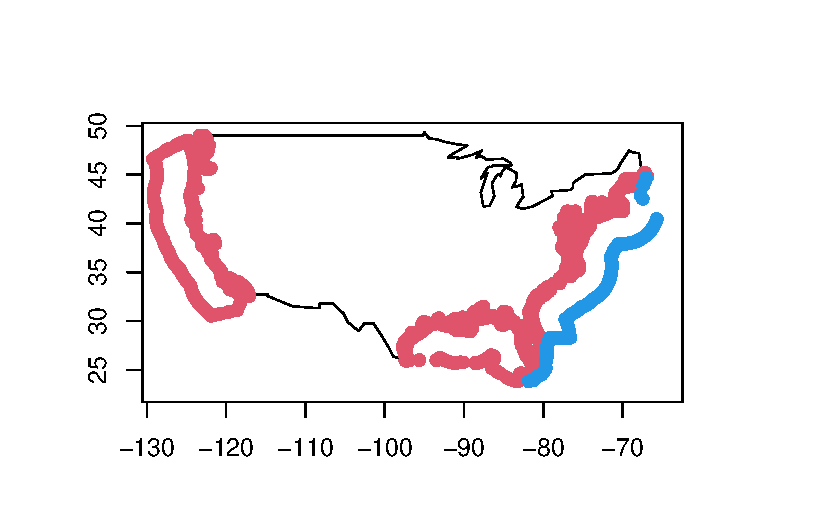
\includegraphics{makeEEZ_files/figure-pdf/unnamed-chunk-1-1.pdf}

\subsection{Construct the U.S. EEZ}\label{construct-the-u.s.-eez}

We simplify the shapefile along the U.S. coast in order to simplify
computations later in the process.

\begin{Shaded}
\begin{Highlighting}[]
\CommentTok{\# subset points N and S of 35N for later delineation}
\NormalTok{co2 }\OtherTok{\textless{}{-}}\NormalTok{ co[}\SpecialCharTok{{-}}\FunctionTok{c}\NormalTok{(}\DecValTok{2100}\SpecialCharTok{:}\DecValTok{3727}\NormalTok{), ]}
\NormalTok{co3 }\OtherTok{\textless{}{-}}\NormalTok{ co2[}\FunctionTok{which}\NormalTok{(co2}\SpecialCharTok{$}\NormalTok{Y }\SpecialCharTok{\textgreater{}} \DecValTok{35}\NormalTok{), ]}
\NormalTok{co4 }\OtherTok{\textless{}{-}}\NormalTok{ co2[}\FunctionTok{which}\NormalTok{(co2}\SpecialCharTok{$}\NormalTok{Y }\SpecialCharTok{\textless{}=} \DecValTok{35}\NormalTok{), ]}

\CommentTok{\# reduce number of points along the coast to make computation easier}
\NormalTok{co3 }\OtherTok{\textless{}{-}}\NormalTok{ co3[}\FunctionTok{seq}\NormalTok{(}\DecValTok{1}\NormalTok{, }\FunctionTok{nrow}\NormalTok{(co3), }\DecValTok{1100}\NormalTok{), ]}
\NormalTok{co4 }\OtherTok{\textless{}{-}}\NormalTok{ co4[}\FunctionTok{seq}\NormalTok{(}\DecValTok{1}\NormalTok{, }\FunctionTok{nrow}\NormalTok{(co4), }\DecValTok{800}\NormalTok{), ]}

\FunctionTok{map}\NormalTok{(}\StringTok{"usa"}\NormalTok{, }\AttributeTok{xlim =} \FunctionTok{c}\NormalTok{(}\SpecialCharTok{{-}}\DecValTok{100}\NormalTok{, }\SpecialCharTok{{-}}\DecValTok{60}\NormalTok{), }\AttributeTok{ylim =} \FunctionTok{c}\NormalTok{(}\DecValTok{23}\NormalTok{, }\DecValTok{50}\NormalTok{))}
\FunctionTok{axis}\NormalTok{(}\DecValTok{1}\NormalTok{); }\FunctionTok{axis}\NormalTok{(}\DecValTok{2}\NormalTok{); }\FunctionTok{box}\NormalTok{()}
\FunctionTok{points}\NormalTok{(co3}\SpecialCharTok{$}\NormalTok{X, co3}\SpecialCharTok{$}\NormalTok{Y, }\AttributeTok{col =} \DecValTok{2}\NormalTok{, }\AttributeTok{pch =} \DecValTok{19}\NormalTok{)}
\FunctionTok{points}\NormalTok{(co4}\SpecialCharTok{$}\NormalTok{X, co4}\SpecialCharTok{$}\NormalTok{Y, }\AttributeTok{col =} \DecValTok{4}\NormalTok{, }\AttributeTok{pch =} \DecValTok{19}\NormalTok{)}

\NormalTok{co2 }\OtherTok{\textless{}{-}} \FunctionTok{rbind}\NormalTok{(co3, co4)}
\NormalTok{co2 }\OtherTok{\textless{}{-}}\NormalTok{ co2[}\FunctionTok{order}\NormalTok{(co2}\SpecialCharTok{$}\NormalTok{Y), ]}
\NormalTok{cofin }\OtherTok{\textless{}{-}} \FunctionTok{rbind}\NormalTok{(co1, co2)}

\FunctionTok{polygon}\NormalTok{(cofin}\SpecialCharTok{$}\NormalTok{X, cofin}\SpecialCharTok{$}\NormalTok{Y, }\AttributeTok{border =} \DecValTok{5}\NormalTok{, }\AttributeTok{lwd =} \DecValTok{3}\NormalTok{)}

\CommentTok{\# make the polygon along the coast line a bit more linear}
\FunctionTok{abline}\NormalTok{(}\AttributeTok{h =} \FloatTok{37.5}\NormalTok{)}
\FunctionTok{abline}\NormalTok{(}\AttributeTok{v =} \SpecialCharTok{{-}}\DecValTok{74}\NormalTok{)}
\end{Highlighting}
\end{Shaded}

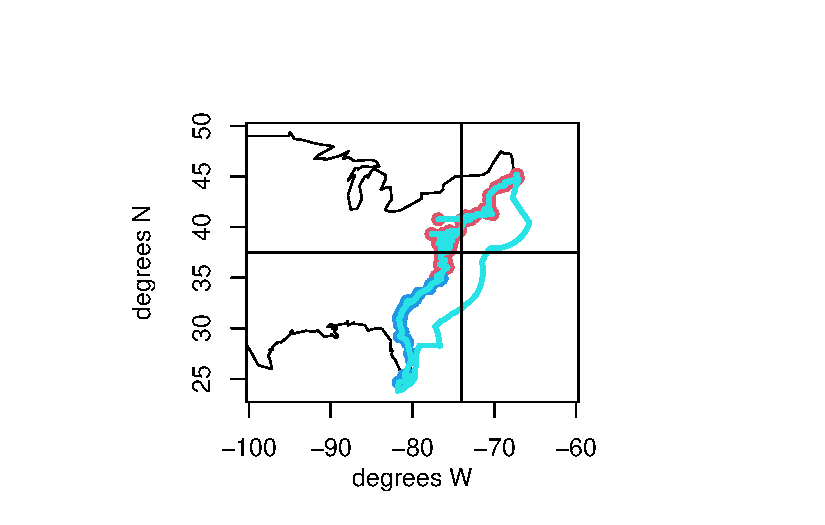
\includegraphics{makeEEZ_files/figure-pdf/unnamed-chunk-2-1.pdf}

\begin{Shaded}
\begin{Highlighting}[]
\NormalTok{cofin }\OtherTok{\textless{}{-}}\NormalTok{ cofin[}\SpecialCharTok{{-}}\FunctionTok{which}\NormalTok{(cofin}\SpecialCharTok{$}\NormalTok{X }\SpecialCharTok{\textless{}}\NormalTok{ (}\SpecialCharTok{{-}}\DecValTok{74}\NormalTok{) }\SpecialCharTok{\&}\NormalTok{ cofin}\SpecialCharTok{$}\NormalTok{Y }\SpecialCharTok{\textgreater{}} \FloatTok{37.6}\NormalTok{), ]}
\CommentTok{\#text(cofin$X, cofin$Y, 1:nrow(cofin), cex = 0.9)}
\NormalTok{lis }\OtherTok{\textless{}{-}} \FunctionTok{c}\NormalTok{(}\DecValTok{1634}\NormalTok{, }\DecValTok{1639}\NormalTok{, }\DecValTok{1688}\NormalTok{, }\DecValTok{1710}\NormalTok{, }\DecValTok{1711}\NormalTok{, }\DecValTok{1712}\NormalTok{)}
\NormalTok{cofin }\OtherTok{\textless{}{-}}\NormalTok{ cofin[}\SpecialCharTok{{-}}\NormalTok{lis, ]}

\FunctionTok{map}\NormalTok{(}\AttributeTok{database =} \StringTok{"usa"}\NormalTok{, }\AttributeTok{xlim =} \FunctionTok{c}\NormalTok{(}\SpecialCharTok{{-}}\DecValTok{70}\NormalTok{, }\SpecialCharTok{{-}}\DecValTok{65}\NormalTok{), }\AttributeTok{ylim =} \FunctionTok{c}\NormalTok{(}\DecValTok{43}\NormalTok{, }\DecValTok{47}\NormalTok{), }\AttributeTok{col =} \DecValTok{8}\NormalTok{)}
\FunctionTok{axis}\NormalTok{(}\DecValTok{1}\NormalTok{); }\FunctionTok{axis}\NormalTok{(}\DecValTok{2}\NormalTok{)}
\FunctionTok{polygon}\NormalTok{(cofin}\SpecialCharTok{$}\NormalTok{X, cofin}\SpecialCharTok{$}\NormalTok{Y, }\AttributeTok{border =} \DecValTok{2}\NormalTok{, }\AttributeTok{lwd =} \DecValTok{2}\NormalTok{)}
\FunctionTok{text}\NormalTok{(cofin}\SpecialCharTok{$}\NormalTok{X, cofin}\SpecialCharTok{$}\NormalTok{Y, }\DecValTok{1}\SpecialCharTok{:}\FunctionTok{nrow}\NormalTok{(cofin), }\AttributeTok{cex =} \FloatTok{0.9}\NormalTok{)}
\end{Highlighting}
\end{Shaded}

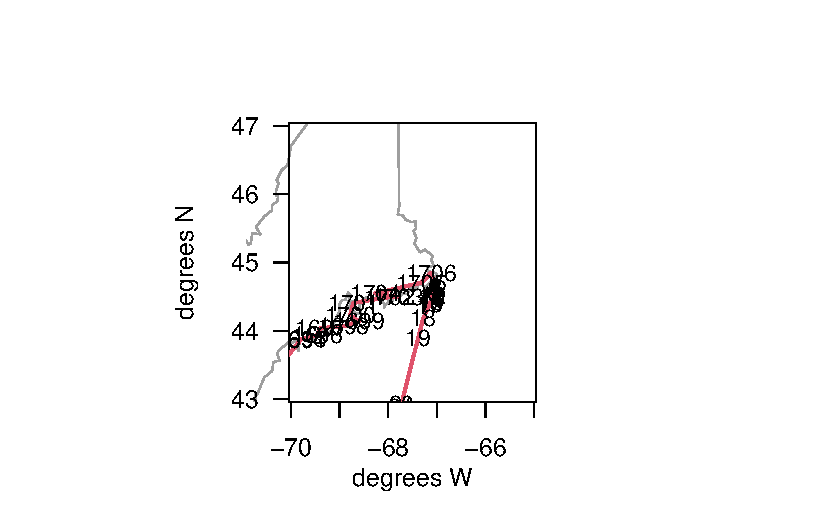
\includegraphics{makeEEZ_files/figure-pdf/unnamed-chunk-2-2.pdf}

\begin{Shaded}
\begin{Highlighting}[]
\FunctionTok{map}\NormalTok{(}\AttributeTok{database =} \StringTok{"usa"}\NormalTok{, }\AttributeTok{xlim =} \FunctionTok{c}\NormalTok{(}\SpecialCharTok{{-}}\DecValTok{72}\NormalTok{, }\SpecialCharTok{{-}}\DecValTok{71}\NormalTok{), }\AttributeTok{ylim =} \FunctionTok{c}\NormalTok{(}\FloatTok{34.8}\NormalTok{, }\FloatTok{35.1}\NormalTok{))}
\FunctionTok{axis}\NormalTok{(}\DecValTok{1}\NormalTok{); }\FunctionTok{axis}\NormalTok{(}\DecValTok{2}\NormalTok{)}
\FunctionTok{polygon}\NormalTok{(cofin}\SpecialCharTok{$}\NormalTok{X, cofin}\SpecialCharTok{$}\NormalTok{Y, }\AttributeTok{border =} \DecValTok{2}\NormalTok{)}
\FunctionTok{text}\NormalTok{(cofin}\SpecialCharTok{$}\NormalTok{X, cofin}\SpecialCharTok{$}\NormalTok{Y, }\DecValTok{1}\SpecialCharTok{:}\FunctionTok{nrow}\NormalTok{(cofin), }\AttributeTok{cex =} \FloatTok{0.6}\NormalTok{)}
\FunctionTok{abline}\NormalTok{(}\AttributeTok{h=}\DecValTok{35}\NormalTok{)}
\FunctionTok{abline}\NormalTok{(}\AttributeTok{v =} \SpecialCharTok{{-}}\DecValTok{60}\NormalTok{)}
\end{Highlighting}
\end{Shaded}

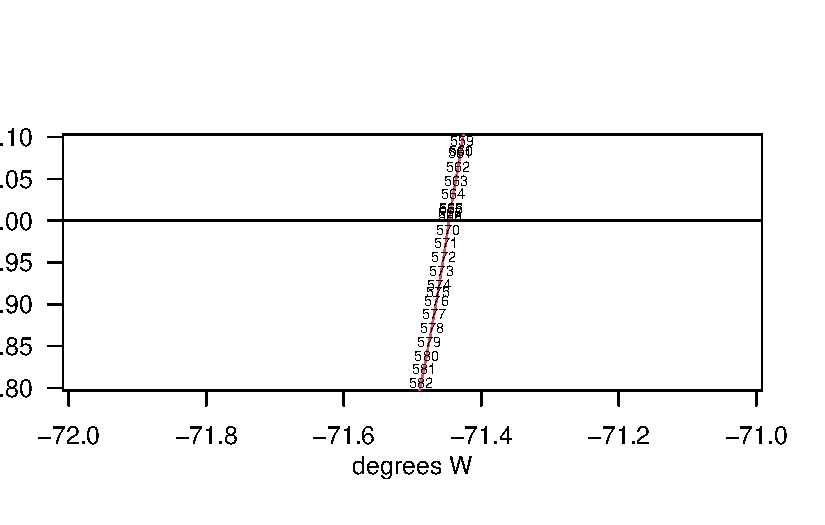
\includegraphics{makeEEZ_files/figure-pdf/unnamed-chunk-2-3.pdf}

\begin{Shaded}
\begin{Highlighting}[]
\NormalTok{cofin }\OtherTok{\textless{}{-}}\NormalTok{ cofin[, }\DecValTok{1}\SpecialCharTok{:}\DecValTok{2}\NormalTok{]}

\FunctionTok{map}\NormalTok{(}\AttributeTok{database =} \StringTok{"usa"}\NormalTok{, }\AttributeTok{xlim =} \FunctionTok{c}\NormalTok{(}\SpecialCharTok{{-}}\DecValTok{83}\NormalTok{, }\SpecialCharTok{{-}}\DecValTok{60}\NormalTok{), }\AttributeTok{ylim =} \FunctionTok{c}\NormalTok{(}\DecValTok{23}\NormalTok{, }\DecValTok{47}\NormalTok{))}
\FunctionTok{axis}\NormalTok{(}\DecValTok{1}\NormalTok{); }\FunctionTok{axis}\NormalTok{(}\DecValTok{2}\NormalTok{)}
\FunctionTok{polygon}\NormalTok{(cofin}\SpecialCharTok{$}\NormalTok{X, cofin}\SpecialCharTok{$}\NormalTok{Y, }\AttributeTok{border =} \DecValTok{2}\NormalTok{)}
\end{Highlighting}
\end{Shaded}

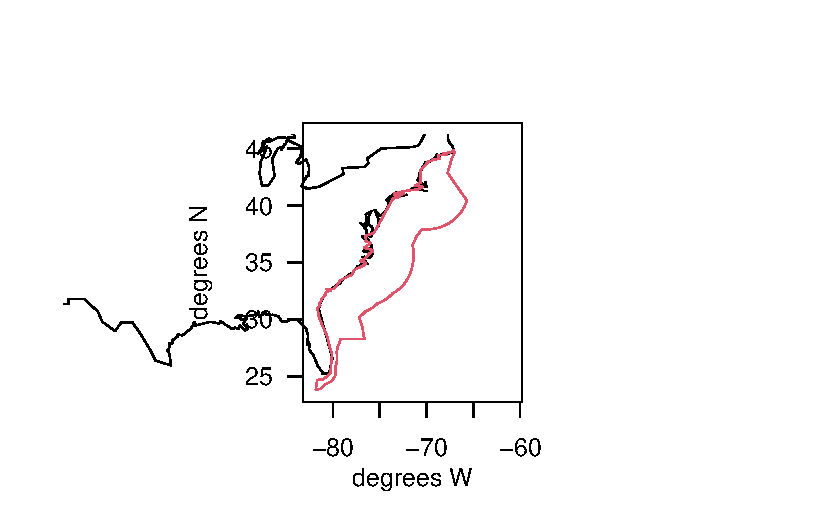
\includegraphics{makeEEZ_files/figure-pdf/unnamed-chunk-2-4.pdf}

\begin{Shaded}
\begin{Highlighting}[]
\CommentTok{\# change the southernmost tip to exactly 24N so that it alighs with Caribbean polygon}
\NormalTok{cofin }\OtherTok{\textless{}{-}}\NormalTok{ cofin[}\SpecialCharTok{{-}}\FunctionTok{which}\NormalTok{(cofin}\SpecialCharTok{$}\NormalTok{Y }\SpecialCharTok{\textless{}} \DecValTok{24}\NormalTok{), ]}
\NormalTok{cofin[}\DecValTok{1624}\NormalTok{, }\DecValTok{2}\NormalTok{] }\OtherTok{\textless{}{-}} \DecValTok{24}

\NormalTok{USeez }\OtherTok{\textless{}{-}}\NormalTok{ cofin}
\CommentTok{\#write.csv(USeez, file = "eez.csv")}
\end{Highlighting}
\end{Shaded}

Here is a final U.S. South Atlantic EEZ polygon, with a simplified
coastline to reduce computational time when subsetting data points.

\subsection{Define the Caribbean
region}\label{define-the-caribbean-region}

Now we define the boundaries of the Caribbean region. Its northernmost
boundary aligns with the EEZ along Florida's coast up to 28.3 degrees N,
at which point the boundary cuts southeast until it intersects with the
24N boundary just east of the Bahamas, approximating the Bahamas EEX.
Its western boundary is -90 degrees W and its southern boundary is 8
degrees N (essentially the land boundary of the Caribbean Sea). Its
eastern boundary is -71.1 degrees W.

\begin{Shaded}
\begin{Highlighting}[]
\FunctionTok{which.min}\NormalTok{(cofin}\SpecialCharTok{$}\NormalTok{Y)}
\end{Highlighting}
\end{Shaded}

\begin{verbatim}
[1] 1624
\end{verbatim}

\begin{Shaded}
\begin{Highlighting}[]
\NormalTok{cofin[}\DecValTok{1624}\NormalTok{, ]}
\end{Highlighting}
\end{Shaded}

\begin{verbatim}
             X  Y
3723 -81.16148 24
\end{verbatim}

\begin{Shaded}
\begin{Highlighting}[]
\FunctionTok{map}\NormalTok{(}\AttributeTok{database =} \StringTok{"usa"}\NormalTok{, }\AttributeTok{xlim =} \FunctionTok{c}\NormalTok{(}\SpecialCharTok{{-}}\DecValTok{77}\NormalTok{, }\SpecialCharTok{{-}}\FloatTok{76.4}\NormalTok{), }\AttributeTok{ylim =} \FunctionTok{c}\NormalTok{(}\DecValTok{28}\NormalTok{, }\FloatTok{28.9}\NormalTok{))}
\FunctionTok{axis}\NormalTok{(}\DecValTok{1}\NormalTok{); }\FunctionTok{axis}\NormalTok{(}\DecValTok{2}\NormalTok{, }\AttributeTok{las =} \DecValTok{2}\NormalTok{); }\FunctionTok{box}\NormalTok{()}
\FunctionTok{polygon}\NormalTok{(cofin}\SpecialCharTok{$}\NormalTok{X, cofin}\SpecialCharTok{$}\NormalTok{Y, }\AttributeTok{border =} \DecValTok{2}\NormalTok{)}
\FunctionTok{text}\NormalTok{(cofin}\SpecialCharTok{$}\NormalTok{X, cofin}\SpecialCharTok{$}\NormalTok{Y, }\DecValTok{1}\SpecialCharTok{:}\FunctionTok{nrow}\NormalTok{(cofin), }\AttributeTok{cex =} \FloatTok{0.6}\NormalTok{)}
\end{Highlighting}
\end{Shaded}

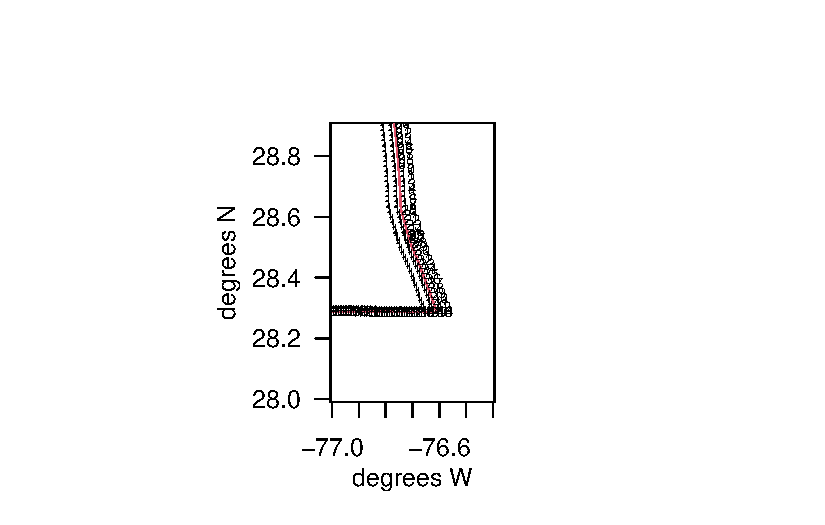
\includegraphics{makeEEZ_files/figure-pdf/unnamed-chunk-3-1.pdf}

\begin{Shaded}
\begin{Highlighting}[]
\NormalTok{car1 }\OtherTok{\textless{}{-}}\NormalTok{ cofin[}\DecValTok{1143}\SpecialCharTok{:}\DecValTok{1624}\NormalTok{, ]}
\NormalTok{car2 }\OtherTok{\textless{}{-}} \FunctionTok{data.frame}\NormalTok{(}\FunctionTok{cbind}\NormalTok{(}\FunctionTok{c}\NormalTok{(}\SpecialCharTok{{-}}\DecValTok{90}\NormalTok{, }\SpecialCharTok{{-}}\DecValTok{90}\NormalTok{, }\SpecialCharTok{{-}}\DecValTok{60}\NormalTok{, }\SpecialCharTok{{-}}\DecValTok{60}\NormalTok{, }\SpecialCharTok{{-}}\FloatTok{71.1}\NormalTok{), }\FunctionTok{c}\NormalTok{(}\DecValTok{24}\NormalTok{, }\DecValTok{8}\NormalTok{, }\DecValTok{8}\NormalTok{, }\DecValTok{24}\NormalTok{, }\DecValTok{24}\NormalTok{)))}
\FunctionTok{names}\NormalTok{(car2) }\OtherTok{\textless{}{-}} \FunctionTok{c}\NormalTok{(}\StringTok{"X"}\NormalTok{, }\StringTok{"Y"}\NormalTok{)}
\NormalTok{CAR }\OtherTok{\textless{}{-}} \FunctionTok{rbind}\NormalTok{(car1, car2)}
\FunctionTok{names}\NormalTok{(CAR) }\OtherTok{\textless{}{-}} \FunctionTok{c}\NormalTok{(}\StringTok{"X"}\NormalTok{, }\StringTok{"Y"}\NormalTok{)}

\FunctionTok{map}\NormalTok{(}\AttributeTok{database =} \StringTok{"usa"}\NormalTok{, }\AttributeTok{xlim =} \FunctionTok{c}\NormalTok{(}\SpecialCharTok{{-}}\DecValTok{95}\NormalTok{, }\SpecialCharTok{{-}}\DecValTok{60}\NormalTok{), }\AttributeTok{ylim =} \FunctionTok{c}\NormalTok{(}\DecValTok{5}\NormalTok{, }\DecValTok{36}\NormalTok{))}
\FunctionTok{axis}\NormalTok{(}\DecValTok{1}\NormalTok{); }\FunctionTok{axis}\NormalTok{(}\DecValTok{2}\NormalTok{, }\AttributeTok{las =} \DecValTok{2}\NormalTok{); }\FunctionTok{box}\NormalTok{()}
\FunctionTok{polygon}\NormalTok{(CAR}\SpecialCharTok{$}\NormalTok{X, CAR}\SpecialCharTok{$}\NormalTok{Y, }\AttributeTok{col =} \DecValTok{2}\NormalTok{)}
\end{Highlighting}
\end{Shaded}

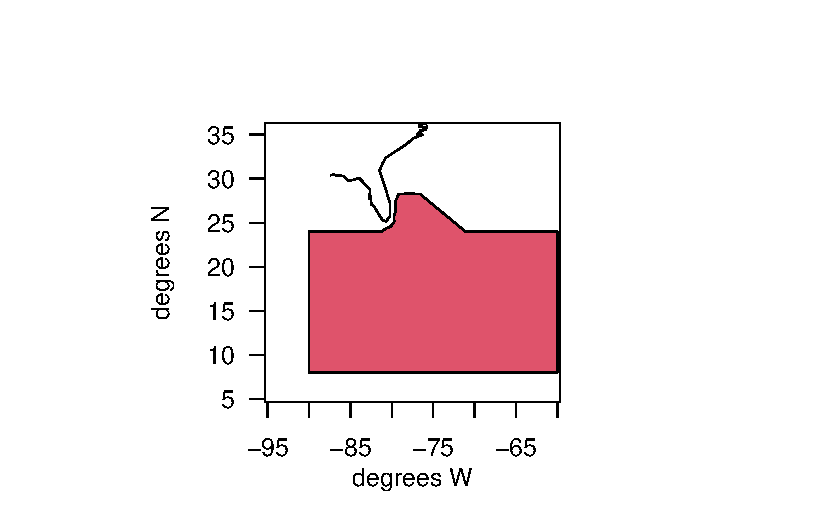
\includegraphics{makeEEZ_files/figure-pdf/unnamed-chunk-3-2.pdf}

\section{Define the NCA region}\label{define-the-nca-region}

The North Central Atlantic (NCA) region, otherwise known as the Western
Central Atlantic, is defined according to the boundaries of FAO area
\href{https://www.fao.org/fishery/en/area/fao:31/en}{31}, but excluding
the U.S. EEZ and Caribbean territorial seas to the West.

\begin{Shaded}
\begin{Highlighting}[]
\NormalTok{nca1 }\OtherTok{\textless{}{-}}\NormalTok{ cofin[}\DecValTok{569}\SpecialCharTok{:}\DecValTok{1143}\NormalTok{, ]  }\CommentTok{\# subset points along EEZ}
\NormalTok{nca2 }\OtherTok{\textless{}{-}} \FunctionTok{data.frame}\NormalTok{(}\FunctionTok{cbind}\NormalTok{(}\FunctionTok{c}\NormalTok{(}\SpecialCharTok{{-}}\FloatTok{71.1}\NormalTok{, }\SpecialCharTok{{-}}\DecValTok{60}\NormalTok{, }\SpecialCharTok{{-}}\DecValTok{60}\NormalTok{, }\SpecialCharTok{{-}}\DecValTok{40}\NormalTok{, }\SpecialCharTok{{-}}\DecValTok{40}\NormalTok{), }\FunctionTok{c}\NormalTok{(}\DecValTok{24}\NormalTok{, }\DecValTok{24}\NormalTok{, }\DecValTok{13}\NormalTok{, }\DecValTok{13}\NormalTok{, }\DecValTok{35}\NormalTok{))) }\CommentTok{\# define boundaries according to FAO}
\FunctionTok{names}\NormalTok{(nca2) }\OtherTok{\textless{}{-}} \FunctionTok{c}\NormalTok{(}\StringTok{"X"}\NormalTok{, }\StringTok{"Y"}\NormalTok{)}
\NormalTok{NCA }\OtherTok{\textless{}{-}} \FunctionTok{rbind}\NormalTok{(nca1, nca2)}
\FunctionTok{names}\NormalTok{(NCA) }\OtherTok{\textless{}{-}} \FunctionTok{c}\NormalTok{(}\StringTok{"X"}\NormalTok{, }\StringTok{"Y"}\NormalTok{)}

\FunctionTok{map}\NormalTok{(}\AttributeTok{database =} \StringTok{"usa"}\NormalTok{, }\AttributeTok{xlim =} \FunctionTok{c}\NormalTok{(}\SpecialCharTok{{-}}\DecValTok{85}\NormalTok{, }\SpecialCharTok{{-}}\DecValTok{30}\NormalTok{), }\AttributeTok{ylim =} \FunctionTok{c}\NormalTok{(}\DecValTok{10}\NormalTok{, }\DecValTok{36}\NormalTok{))}
\FunctionTok{axis}\NormalTok{(}\DecValTok{1}\NormalTok{); }\FunctionTok{axis}\NormalTok{(}\DecValTok{2}\NormalTok{, }\AttributeTok{las =} \DecValTok{2}\NormalTok{); }\FunctionTok{box}\NormalTok{()}
\FunctionTok{polygon}\NormalTok{(NCA}\SpecialCharTok{$}\NormalTok{X, NCA}\SpecialCharTok{$}\NormalTok{Y, }\AttributeTok{col =} \DecValTok{3}\NormalTok{)}
\end{Highlighting}
\end{Shaded}

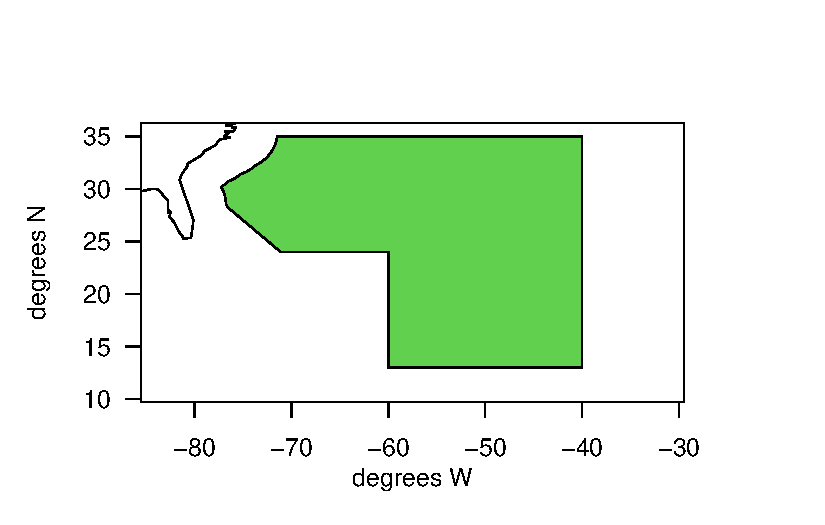
\includegraphics{makeEEZ_files/figure-pdf/unnamed-chunk-4-1.pdf}

\section{Define the NED region}\label{define-the-ned-region}

The Northeast Distant Waters (NED) region, otherwise known as the
Northwesetern Atlantic, is defined according to the boundaries of FAO
area \href{https://www.fao.org/fishery/en/area/fao:21/en}{21}, but
excluding the U.S. EEZ territorial seas to the West. It does include
Canadian and French territorial EEZs. The northern boundary is 60
degrees north, as dolphin are not caught above this latitude.

\begin{Shaded}
\begin{Highlighting}[]
\FunctionTok{which.max}\NormalTok{(cofin}\SpecialCharTok{$}\NormalTok{Y)  }\CommentTok{\# find northernmost point of U.S. EEZ}
\end{Highlighting}
\end{Shaded}

\begin{verbatim}
[1] 1702
\end{verbatim}

\begin{Shaded}
\begin{Highlighting}[]
\NormalTok{cofin[}\DecValTok{1702}\NormalTok{, ]}
\end{Highlighting}
\end{Shaded}

\begin{verbatim}
              X        Y
77844 -67.11553 44.84764
\end{verbatim}

\begin{Shaded}
\begin{Highlighting}[]
\NormalTok{ned1 }\OtherTok{\textless{}{-}}\NormalTok{ cofin[}\DecValTok{1}\SpecialCharTok{:}\DecValTok{569}\NormalTok{, ]  }\CommentTok{\# subset points along EEZ}
\NormalTok{ned2 }\OtherTok{\textless{}{-}} \FunctionTok{data.frame}\NormalTok{(}\FunctionTok{cbind}\NormalTok{(}\FunctionTok{c}\NormalTok{(}\SpecialCharTok{{-}}\DecValTok{42}\NormalTok{, }\SpecialCharTok{{-}}\DecValTok{42}\NormalTok{, }\SpecialCharTok{{-}}\FloatTok{67.1}\NormalTok{), }\FunctionTok{c}\NormalTok{(}\DecValTok{35}\NormalTok{, }\DecValTok{55}\NormalTok{, }\DecValTok{55}\NormalTok{)))  }\CommentTok{\# define boundaries according to FAO}
\FunctionTok{names}\NormalTok{(ned2) }\OtherTok{\textless{}{-}} \FunctionTok{c}\NormalTok{(}\StringTok{"X"}\NormalTok{, }\StringTok{"Y"}\NormalTok{)}
\NormalTok{NED }\OtherTok{\textless{}{-}} \FunctionTok{rbind}\NormalTok{(ned1, ned2)}
\FunctionTok{names}\NormalTok{(NED) }\OtherTok{\textless{}{-}} \FunctionTok{c}\NormalTok{(}\StringTok{"X"}\NormalTok{, }\StringTok{"Y"}\NormalTok{)}

\FunctionTok{map}\NormalTok{(}\AttributeTok{database =} \StringTok{"usa"}\NormalTok{, }\AttributeTok{xlim =} \FunctionTok{c}\NormalTok{(}\SpecialCharTok{{-}}\DecValTok{85}\NormalTok{, }\SpecialCharTok{{-}}\DecValTok{30}\NormalTok{), }\AttributeTok{ylim =} \FunctionTok{c}\NormalTok{(}\DecValTok{30}\NormalTok{, }\DecValTok{60}\NormalTok{))}
\FunctionTok{axis}\NormalTok{(}\DecValTok{1}\NormalTok{); }\FunctionTok{axis}\NormalTok{(}\DecValTok{2}\NormalTok{, }\AttributeTok{las =} \DecValTok{2}\NormalTok{); }\FunctionTok{box}\NormalTok{()}
\FunctionTok{polygon}\NormalTok{(NED}\SpecialCharTok{$}\NormalTok{X, NED}\SpecialCharTok{$}\NormalTok{Y, }\AttributeTok{col =} \DecValTok{4}\NormalTok{)}
\end{Highlighting}
\end{Shaded}

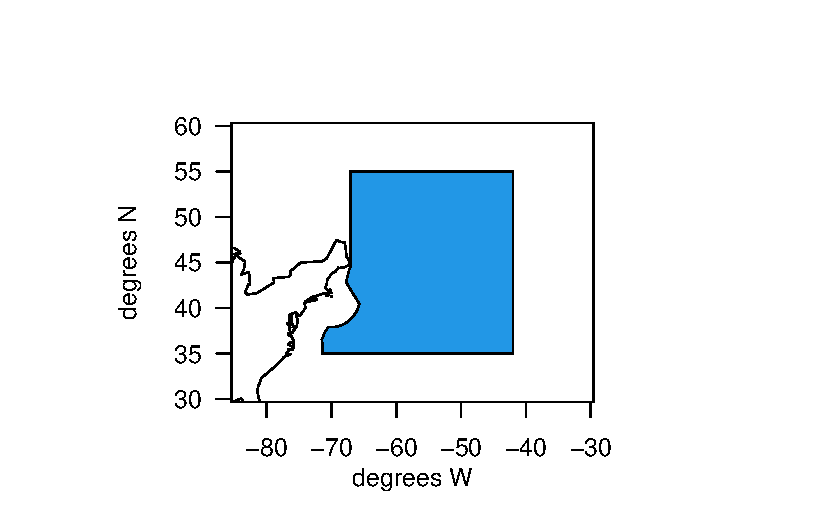
\includegraphics{makeEEZ_files/figure-pdf/unnamed-chunk-5-1.pdf}

\section{Define the Florida Keys
region}\label{define-the-florida-keys-region}

The southernmost region of the U.S. EEZ is called the FLK region, and
includes waters within the EEZ boundary, north up to 28 degrees N. The
boundary of 28N is chosen because it aligns with commercial logbook
reporting boundaries and aligns roughly with the Brevard - Indian River
County border. This is convenient because U.S. recreational statistics
are summarized as groups of counties, with SE FL encompassing Miami-Dade
to Indian River County and NE FL encompassing Brevard to Nassau County.

\begin{Shaded}
\begin{Highlighting}[]
\FunctionTok{which.min}\NormalTok{(}\FunctionTok{abs}\NormalTok{(co1}\SpecialCharTok{$}\NormalTok{Y }\SpecialCharTok{{-}} \DecValTok{28}\NormalTok{))  }\CommentTok{\# find the southernmost point}
\end{Highlighting}
\end{Shaded}

\begin{verbatim}
[1] 1289
\end{verbatim}

\begin{Shaded}
\begin{Highlighting}[]
\FunctionTok{map}\NormalTok{(}\AttributeTok{database =} \StringTok{"usa"}\NormalTok{, }\AttributeTok{xlim =} \FunctionTok{c}\NormalTok{(}\SpecialCharTok{{-}}\DecValTok{81}\NormalTok{, }\SpecialCharTok{{-}}\DecValTok{78}\NormalTok{), }\AttributeTok{ylim =} \FunctionTok{c}\NormalTok{(}\FloatTok{27.5}\NormalTok{, }\FloatTok{28.9}\NormalTok{))}
\FunctionTok{axis}\NormalTok{(}\DecValTok{1}\NormalTok{); }\FunctionTok{axis}\NormalTok{(}\DecValTok{2}\NormalTok{)}
\FunctionTok{polygon}\NormalTok{(cofin}\SpecialCharTok{$}\NormalTok{X, cofin}\SpecialCharTok{$}\NormalTok{Y, }\AttributeTok{border =} \DecValTok{2}\NormalTok{) }
\FunctionTok{text}\NormalTok{(cofin}\SpecialCharTok{$}\NormalTok{X, cofin}\SpecialCharTok{$}\NormalTok{Y, }\DecValTok{1}\SpecialCharTok{:}\FunctionTok{nrow}\NormalTok{(cofin), }\AttributeTok{cex =} \FloatTok{0.6}\NormalTok{)   }\CommentTok{\# find points falling at 28N}
\FunctionTok{points}\NormalTok{(}\SpecialCharTok{{-}}\FloatTok{80.46}\NormalTok{, }\DecValTok{28}\NormalTok{)}
\NormalTok{cofin[}\DecValTok{1632}\NormalTok{, ] }\OtherTok{\textless{}{-}} \FunctionTok{c}\NormalTok{(}\SpecialCharTok{{-}}\FloatTok{80.46}\NormalTok{, }\DecValTok{28}\NormalTok{)}
\FunctionTok{abline}\NormalTok{(}\AttributeTok{h =} \DecValTok{28}\NormalTok{)}
\end{Highlighting}
\end{Shaded}

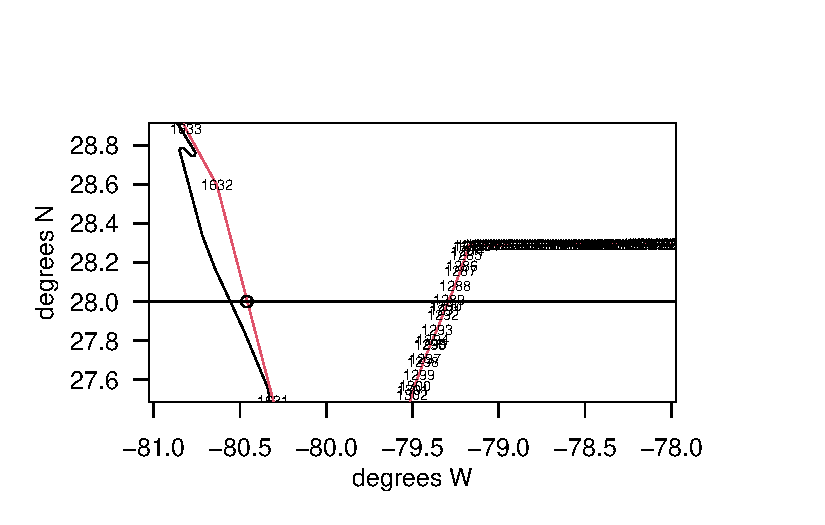
\includegraphics{makeEEZ_files/figure-pdf/unnamed-chunk-6-1.pdf}

\begin{Shaded}
\begin{Highlighting}[]
\NormalTok{FLK }\OtherTok{\textless{}{-}}\NormalTok{ cofin[}\DecValTok{1289}\SpecialCharTok{:}\DecValTok{1632}\NormalTok{, ]  }\CommentTok{\# subset points along EEZ}

\FunctionTok{map}\NormalTok{(}\AttributeTok{database =} \StringTok{"usa"}\NormalTok{, }\AttributeTok{xlim =} \FunctionTok{c}\NormalTok{(}\SpecialCharTok{{-}}\DecValTok{85}\NormalTok{, }\SpecialCharTok{{-}}\DecValTok{75}\NormalTok{), }\AttributeTok{ylim =} \FunctionTok{c}\NormalTok{(}\DecValTok{20}\NormalTok{, }\DecValTok{30}\NormalTok{))}
\FunctionTok{axis}\NormalTok{(}\DecValTok{1}\NormalTok{); }\FunctionTok{axis}\NormalTok{(}\DecValTok{2}\NormalTok{, }\AttributeTok{las =} \DecValTok{2}\NormalTok{); }\FunctionTok{box}\NormalTok{()}
\FunctionTok{polygon}\NormalTok{(FLK}\SpecialCharTok{$}\NormalTok{X, FLK}\SpecialCharTok{$}\NormalTok{Y, }\AttributeTok{col =} \DecValTok{4}\NormalTok{)}
\end{Highlighting}
\end{Shaded}

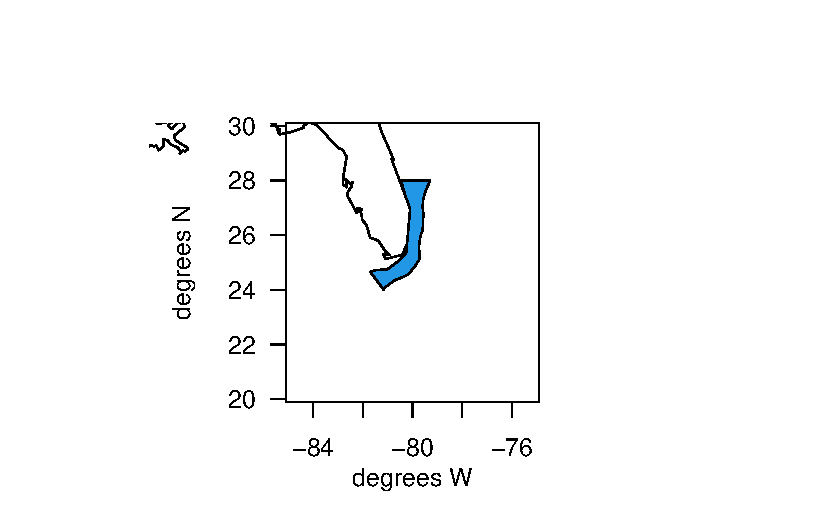
\includegraphics{makeEEZ_files/figure-pdf/unnamed-chunk-6-2.pdf}

\section{Define the North Florida - South NC
region}\label{define-the-north-florida---south-nc-region}

The second area that was decided upon to be defined within the operating
model was northern Florida to Southern North Carolina. We form a
boundary at 35 degrees north because this is the delineation between the
NED and NCA regions. Also, 35N is just south of Cape Hatteras, which is
a boundary for NMFS recreational data collection, as well as a boundary
of commercial logbook data reporting. Therefore, all sources of data
(international, U.S. commercial, and U.S. recreational) can be easily
parsed along this boundary.

\begin{Shaded}
\begin{Highlighting}[]
\FunctionTok{map}\NormalTok{(}\AttributeTok{database =} \StringTok{"usa"}\NormalTok{, }\AttributeTok{xlim =} \FunctionTok{c}\NormalTok{(}\SpecialCharTok{{-}}\DecValTok{72}\NormalTok{, }\SpecialCharTok{{-}}\DecValTok{70}\NormalTok{), }\AttributeTok{ylim =} \FunctionTok{c}\NormalTok{(}\FloatTok{34.5}\NormalTok{, }\FloatTok{35.4}\NormalTok{))}
\FunctionTok{axis}\NormalTok{(}\DecValTok{1}\NormalTok{); }\FunctionTok{axis}\NormalTok{(}\DecValTok{2}\NormalTok{)}
\FunctionTok{polygon}\NormalTok{(cofin}\SpecialCharTok{$}\NormalTok{X, cofin}\SpecialCharTok{$}\NormalTok{Y, }\AttributeTok{border =} \DecValTok{2}\NormalTok{)}
\FunctionTok{text}\NormalTok{(cofin}\SpecialCharTok{$}\NormalTok{X, cofin}\SpecialCharTok{$}\NormalTok{Y, }\DecValTok{1}\SpecialCharTok{:}\FunctionTok{nrow}\NormalTok{(cofin), }\AttributeTok{cex =} \FloatTok{0.6}\NormalTok{)  }\CommentTok{\# find points that fall at 35N}
\FunctionTok{abline}\NormalTok{(}\AttributeTok{h =} \DecValTok{35}\NormalTok{)}
\end{Highlighting}
\end{Shaded}

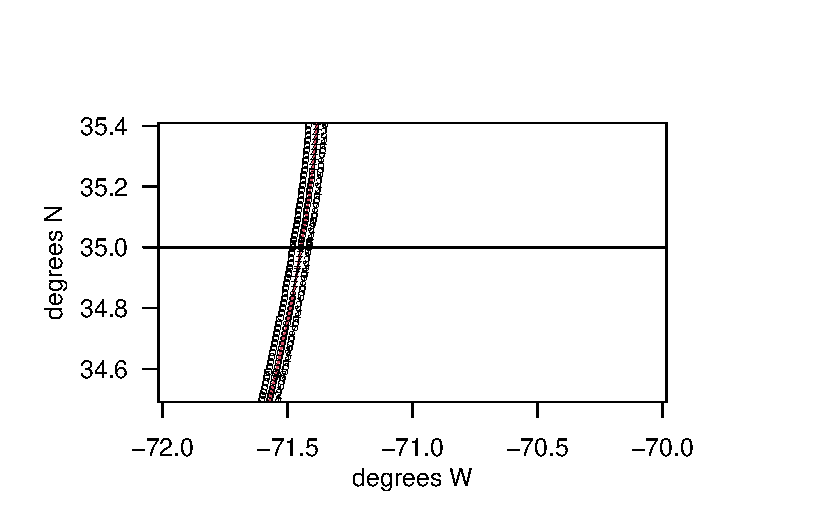
\includegraphics{makeEEZ_files/figure-pdf/unnamed-chunk-7-1.pdf}

\begin{Shaded}
\begin{Highlighting}[]
\NormalTok{cofin[}\DecValTok{1663}\NormalTok{, }\DecValTok{2}\NormalTok{] }\OtherTok{\textless{}{-}} \DecValTok{35}
\NormalTok{NCFL }\OtherTok{\textless{}{-}} \FunctionTok{rbind}\NormalTok{(cofin[}\DecValTok{1632}\SpecialCharTok{:}\DecValTok{1663}\NormalTok{, ], cofin[}\DecValTok{569}\SpecialCharTok{:}\DecValTok{1289}\NormalTok{, ])  }\CommentTok{\# subset along EEZ}

\FunctionTok{map}\NormalTok{(}\AttributeTok{database =} \StringTok{"usa"}\NormalTok{, }\AttributeTok{xlim =} \FunctionTok{c}\NormalTok{(}\SpecialCharTok{{-}}\DecValTok{85}\NormalTok{, }\SpecialCharTok{{-}}\DecValTok{70}\NormalTok{), }\AttributeTok{ylim =} \FunctionTok{c}\NormalTok{(}\DecValTok{25}\NormalTok{, }\DecValTok{40}\NormalTok{))}
\FunctionTok{axis}\NormalTok{(}\DecValTok{1}\NormalTok{); }\FunctionTok{axis}\NormalTok{(}\DecValTok{2}\NormalTok{, }\AttributeTok{las =} \DecValTok{2}\NormalTok{); }\FunctionTok{box}\NormalTok{()}
\FunctionTok{polygon}\NormalTok{(NCFL}\SpecialCharTok{$}\NormalTok{X, NCFL}\SpecialCharTok{$}\NormalTok{Y, }\AttributeTok{col =} \DecValTok{4}\NormalTok{)}
\end{Highlighting}
\end{Shaded}

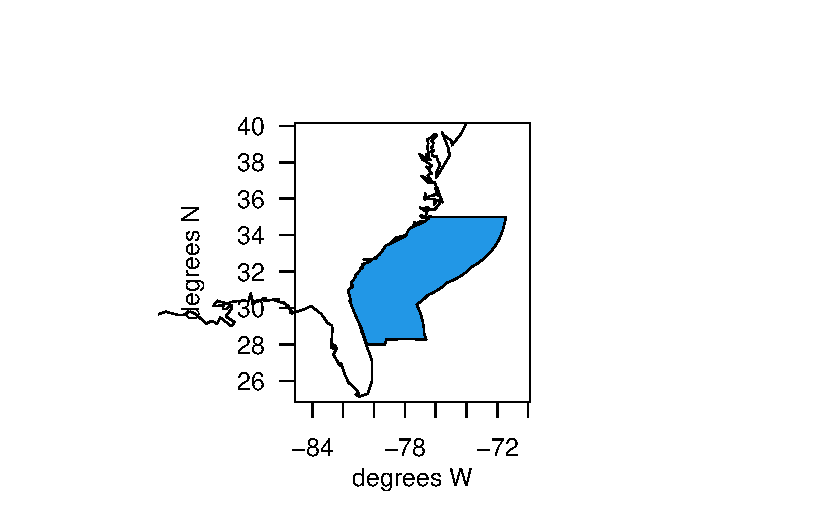
\includegraphics{makeEEZ_files/figure-pdf/unnamed-chunk-7-2.pdf}

\section{Define the northern North Carolina
region}\label{define-the-northern-north-carolina-region}

The third U.S. area that was decided upon to be defined within the
operating model was northern North Carolina, which was intended to
encompass the northern part of the state up to the Virginia border. We
form a boundary at 37 degrees north because this is a boundary for
commercial logbook data reporting and roughly aligns with the latitude
of the state boundary between North Carolina and Virginia. Note there is
a slight misalignment between this boundary and the way that U.S.
recreational statistics are reported (by state), so the commercial and
recreational data will be subset along slightly different boundaries for
this region.

\begin{Shaded}
\begin{Highlighting}[]
\FunctionTok{map}\NormalTok{(}\AttributeTok{database =} \StringTok{"usa"}\NormalTok{, }\AttributeTok{xlim =} \FunctionTok{c}\NormalTok{(}\SpecialCharTok{{-}}\DecValTok{72}\NormalTok{, }\SpecialCharTok{{-}}\DecValTok{70}\NormalTok{), }\AttributeTok{ylim =} \FunctionTok{c}\NormalTok{(}\FloatTok{36.5}\NormalTok{, }\FloatTok{37.4}\NormalTok{))}
\FunctionTok{axis}\NormalTok{(}\DecValTok{1}\NormalTok{); }\FunctionTok{axis}\NormalTok{(}\DecValTok{2}\NormalTok{)}
\FunctionTok{polygon}\NormalTok{(cofin}\SpecialCharTok{$}\NormalTok{X, cofin}\SpecialCharTok{$}\NormalTok{Y, }\AttributeTok{border =} \DecValTok{2}\NormalTok{)}
\FunctionTok{text}\NormalTok{(cofin}\SpecialCharTok{$}\NormalTok{X, cofin}\SpecialCharTok{$}\NormalTok{Y, }\DecValTok{1}\SpecialCharTok{:}\FunctionTok{nrow}\NormalTok{(cofin), }\AttributeTok{cex =} \FloatTok{0.6}\NormalTok{)}
\FunctionTok{abline}\NormalTok{(}\AttributeTok{h =} \DecValTok{37}\NormalTok{)}
\end{Highlighting}
\end{Shaded}

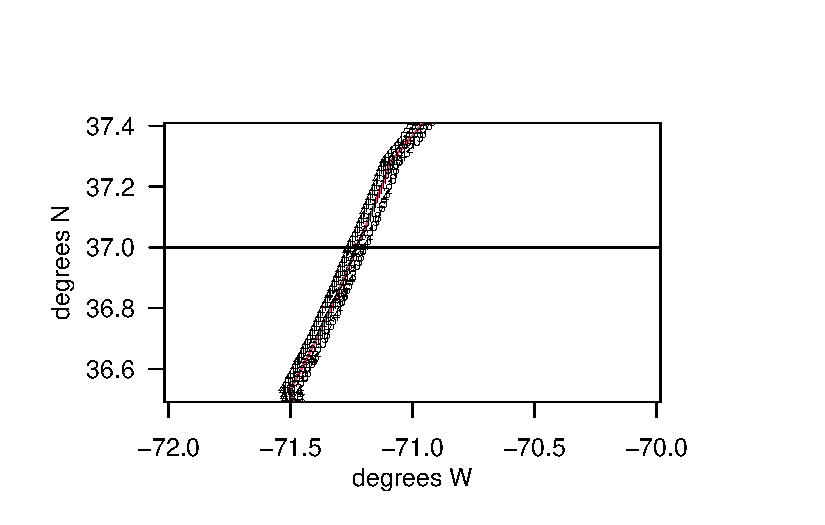
\includegraphics{makeEEZ_files/figure-pdf/unnamed-chunk-8-1.pdf}

\begin{Shaded}
\begin{Highlighting}[]
\NormalTok{cofin[}\DecValTok{425}\NormalTok{, }\DecValTok{2}\NormalTok{] }\OtherTok{\textless{}{-}} \DecValTok{37}
\NormalTok{NNC }\OtherTok{\textless{}{-}} \FunctionTok{rbind}\NormalTok{(cofin[}\DecValTok{1663}\SpecialCharTok{:}\DecValTok{1673}\NormalTok{, ], cofin[}\DecValTok{425}\SpecialCharTok{:}\DecValTok{569}\NormalTok{, ])}

\FunctionTok{map}\NormalTok{(}\AttributeTok{database =} \StringTok{"usa"}\NormalTok{, }\AttributeTok{xlim =} \FunctionTok{c}\NormalTok{(}\SpecialCharTok{{-}}\DecValTok{85}\NormalTok{, }\SpecialCharTok{{-}}\DecValTok{70}\NormalTok{), }\AttributeTok{ylim =} \FunctionTok{c}\NormalTok{(}\DecValTok{25}\NormalTok{, }\DecValTok{40}\NormalTok{))}
\FunctionTok{axis}\NormalTok{(}\DecValTok{1}\NormalTok{); }\FunctionTok{axis}\NormalTok{(}\DecValTok{2}\NormalTok{, }\AttributeTok{las =} \DecValTok{2}\NormalTok{); }\FunctionTok{box}\NormalTok{()}
\FunctionTok{polygon}\NormalTok{(NNC}\SpecialCharTok{$}\NormalTok{X, NNC}\SpecialCharTok{$}\NormalTok{Y, }\AttributeTok{col =} \DecValTok{4}\NormalTok{)}
\end{Highlighting}
\end{Shaded}

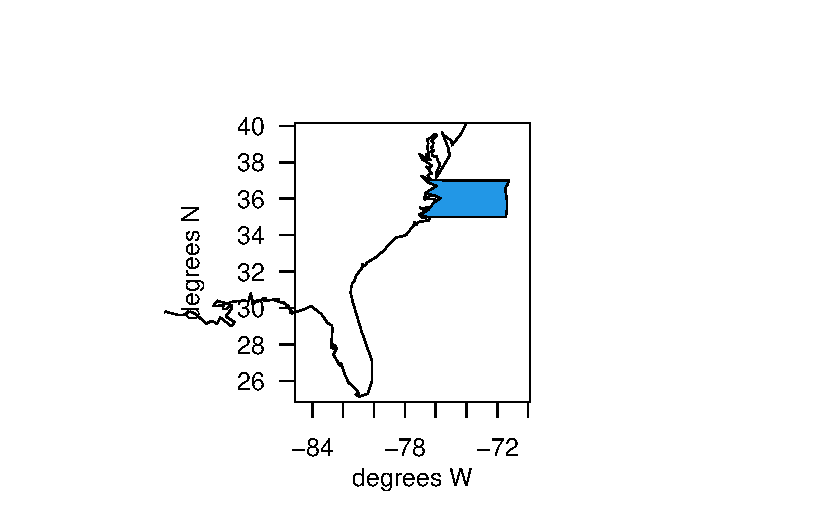
\includegraphics{makeEEZ_files/figure-pdf/unnamed-chunk-8-2.pdf}

\section{Define the Virginia and north
region}\label{define-the-virginia-and-north-region}

The fourth region within the U.S. EEZ is the remainder of the area,
which encompasses national waters from Virginia up to Maine.

\begin{Shaded}
\begin{Highlighting}[]
\NormalTok{VBM }\OtherTok{\textless{}{-}} \FunctionTok{rbind}\NormalTok{(cofin[}\DecValTok{1673}\SpecialCharTok{:}\DecValTok{1702}\NormalTok{, ], cofin[}\DecValTok{1}\SpecialCharTok{:}\DecValTok{425}\NormalTok{, ])}

\FunctionTok{map}\NormalTok{(}\AttributeTok{database =} \StringTok{"usa"}\NormalTok{, }\AttributeTok{xlim =} \FunctionTok{c}\NormalTok{(}\SpecialCharTok{{-}}\DecValTok{80}\NormalTok{, }\SpecialCharTok{{-}}\DecValTok{60}\NormalTok{), }\AttributeTok{ylim =} \FunctionTok{c}\NormalTok{(}\DecValTok{30}\NormalTok{, }\DecValTok{50}\NormalTok{))}
\FunctionTok{axis}\NormalTok{(}\DecValTok{1}\NormalTok{); }\FunctionTok{axis}\NormalTok{(}\DecValTok{2}\NormalTok{, }\AttributeTok{las =} \DecValTok{2}\NormalTok{); }\FunctionTok{box}\NormalTok{()}
\FunctionTok{polygon}\NormalTok{(VBM}\SpecialCharTok{$}\NormalTok{X, VBM}\SpecialCharTok{$}\NormalTok{Y, }\AttributeTok{col =} \DecValTok{4}\NormalTok{)}
\end{Highlighting}
\end{Shaded}

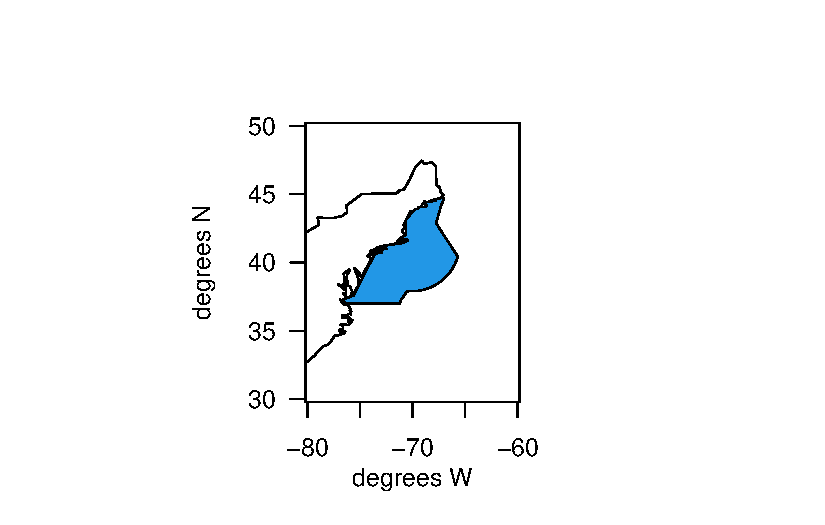
\includegraphics{makeEEZ_files/figure-pdf/unnamed-chunk-9-1.pdf}

\subsection{Plot all of the regions}\label{plot-all-of-the-regions}

Now we will put all of the regions on a single map and check that the
boundaries align.

\begin{Shaded}
\begin{Highlighting}[]
\FunctionTok{map}\NormalTok{(}\AttributeTok{database =} \StringTok{"world"}\NormalTok{, }\AttributeTok{xlim =} \FunctionTok{c}\NormalTok{(}\SpecialCharTok{{-}}\DecValTok{92}\NormalTok{, }\SpecialCharTok{{-}}\DecValTok{38}\NormalTok{), }\AttributeTok{ylim =} \FunctionTok{c}\NormalTok{(}\DecValTok{5}\NormalTok{, }\DecValTok{55}\NormalTok{), }\AttributeTok{col =} \DecValTok{8}\NormalTok{)}
\FunctionTok{axis}\NormalTok{(}\DecValTok{1}\NormalTok{); }\FunctionTok{axis}\NormalTok{(}\DecValTok{2}\NormalTok{, }\AttributeTok{las =} \DecValTok{2}\NormalTok{); }\FunctionTok{box}\NormalTok{()}

\FunctionTok{polygon}\NormalTok{(CAR}\SpecialCharTok{$}\NormalTok{X, CAR}\SpecialCharTok{$}\NormalTok{Y, }\AttributeTok{border =} \DecValTok{1}\NormalTok{)}
\FunctionTok{polygon}\NormalTok{(NCA}\SpecialCharTok{$}\NormalTok{X, NCA}\SpecialCharTok{$}\NormalTok{Y, }\AttributeTok{border =} \DecValTok{1}\NormalTok{)}
\FunctionTok{polygon}\NormalTok{(NED}\SpecialCharTok{$}\NormalTok{X, NED}\SpecialCharTok{$}\NormalTok{Y, }\AttributeTok{border =} \DecValTok{1}\NormalTok{)}
\FunctionTok{polygon}\NormalTok{(FLK}\SpecialCharTok{$}\NormalTok{X, FLK}\SpecialCharTok{$}\NormalTok{Y, }\AttributeTok{border =} \DecValTok{1}\NormalTok{)}
\FunctionTok{polygon}\NormalTok{(NCFL}\SpecialCharTok{$}\NormalTok{X, NCFL}\SpecialCharTok{$}\NormalTok{Y, }\AttributeTok{border =} \DecValTok{1}\NormalTok{)}
\FunctionTok{polygon}\NormalTok{(NNC}\SpecialCharTok{$}\NormalTok{X, NNC}\SpecialCharTok{$}\NormalTok{Y, }\AttributeTok{border =} \DecValTok{1}\NormalTok{)}
\FunctionTok{polygon}\NormalTok{(VBM}\SpecialCharTok{$}\NormalTok{X, VBM}\SpecialCharTok{$}\NormalTok{Y, }\AttributeTok{border =} \DecValTok{1}\NormalTok{)}

\FunctionTok{map}\NormalTok{(}\AttributeTok{database =} \StringTok{"world"}\NormalTok{, }\AttributeTok{add =}\NormalTok{ T, }\AttributeTok{col =} \DecValTok{8}\NormalTok{, }\AttributeTok{lwd =} \DecValTok{2}\NormalTok{)}

\FunctionTok{text}\NormalTok{(}\SpecialCharTok{{-}}\DecValTok{75}\NormalTok{, }\DecValTok{15}\NormalTok{, }\StringTok{"CAR"}\NormalTok{, }\AttributeTok{cex =} \FloatTok{1.2}\NormalTok{)}
\FunctionTok{text}\NormalTok{(}\SpecialCharTok{{-}}\DecValTok{57}\NormalTok{, }\DecValTok{28}\NormalTok{, }\StringTok{"NCA"}\NormalTok{, }\AttributeTok{cex =} \FloatTok{1.2}\NormalTok{)}
\FunctionTok{text}\NormalTok{(}\SpecialCharTok{{-}}\DecValTok{57}\NormalTok{, }\DecValTok{42}\NormalTok{, }\StringTok{"NED"}\NormalTok{, }\AttributeTok{cex =} \FloatTok{1.2}\NormalTok{)}
\FunctionTok{text}\NormalTok{(}\FunctionTok{mean}\NormalTok{(FLK}\SpecialCharTok{$}\NormalTok{X), }\FunctionTok{mean}\NormalTok{(FLK}\SpecialCharTok{$}\NormalTok{Y), }\StringTok{"FLK"}\NormalTok{, }\AttributeTok{cex =} \FloatTok{1.2}\NormalTok{)}
\FunctionTok{text}\NormalTok{(}\SpecialCharTok{{-}}\FloatTok{79.3}\NormalTok{, }\FunctionTok{mean}\NormalTok{(NCFL}\SpecialCharTok{$}\NormalTok{Y), }\StringTok{"NCFL"}\NormalTok{, }\AttributeTok{cex =} \FloatTok{1.2}\NormalTok{)}
\FunctionTok{text}\NormalTok{(}\SpecialCharTok{{-}}\FloatTok{73.8}\NormalTok{, }\FunctionTok{mean}\NormalTok{(NNC}\SpecialCharTok{$}\NormalTok{Y), }\StringTok{"NNC"}\NormalTok{, }\AttributeTok{cex =} \FloatTok{1.2}\NormalTok{)}
\FunctionTok{text}\NormalTok{(}\SpecialCharTok{{-}}\FloatTok{71.5}\NormalTok{, }\FunctionTok{mean}\NormalTok{(VBM}\SpecialCharTok{$}\NormalTok{Y), }\StringTok{"VBM"}\NormalTok{, }\AttributeTok{cex =} \FloatTok{1.2}\NormalTok{)}
\end{Highlighting}
\end{Shaded}

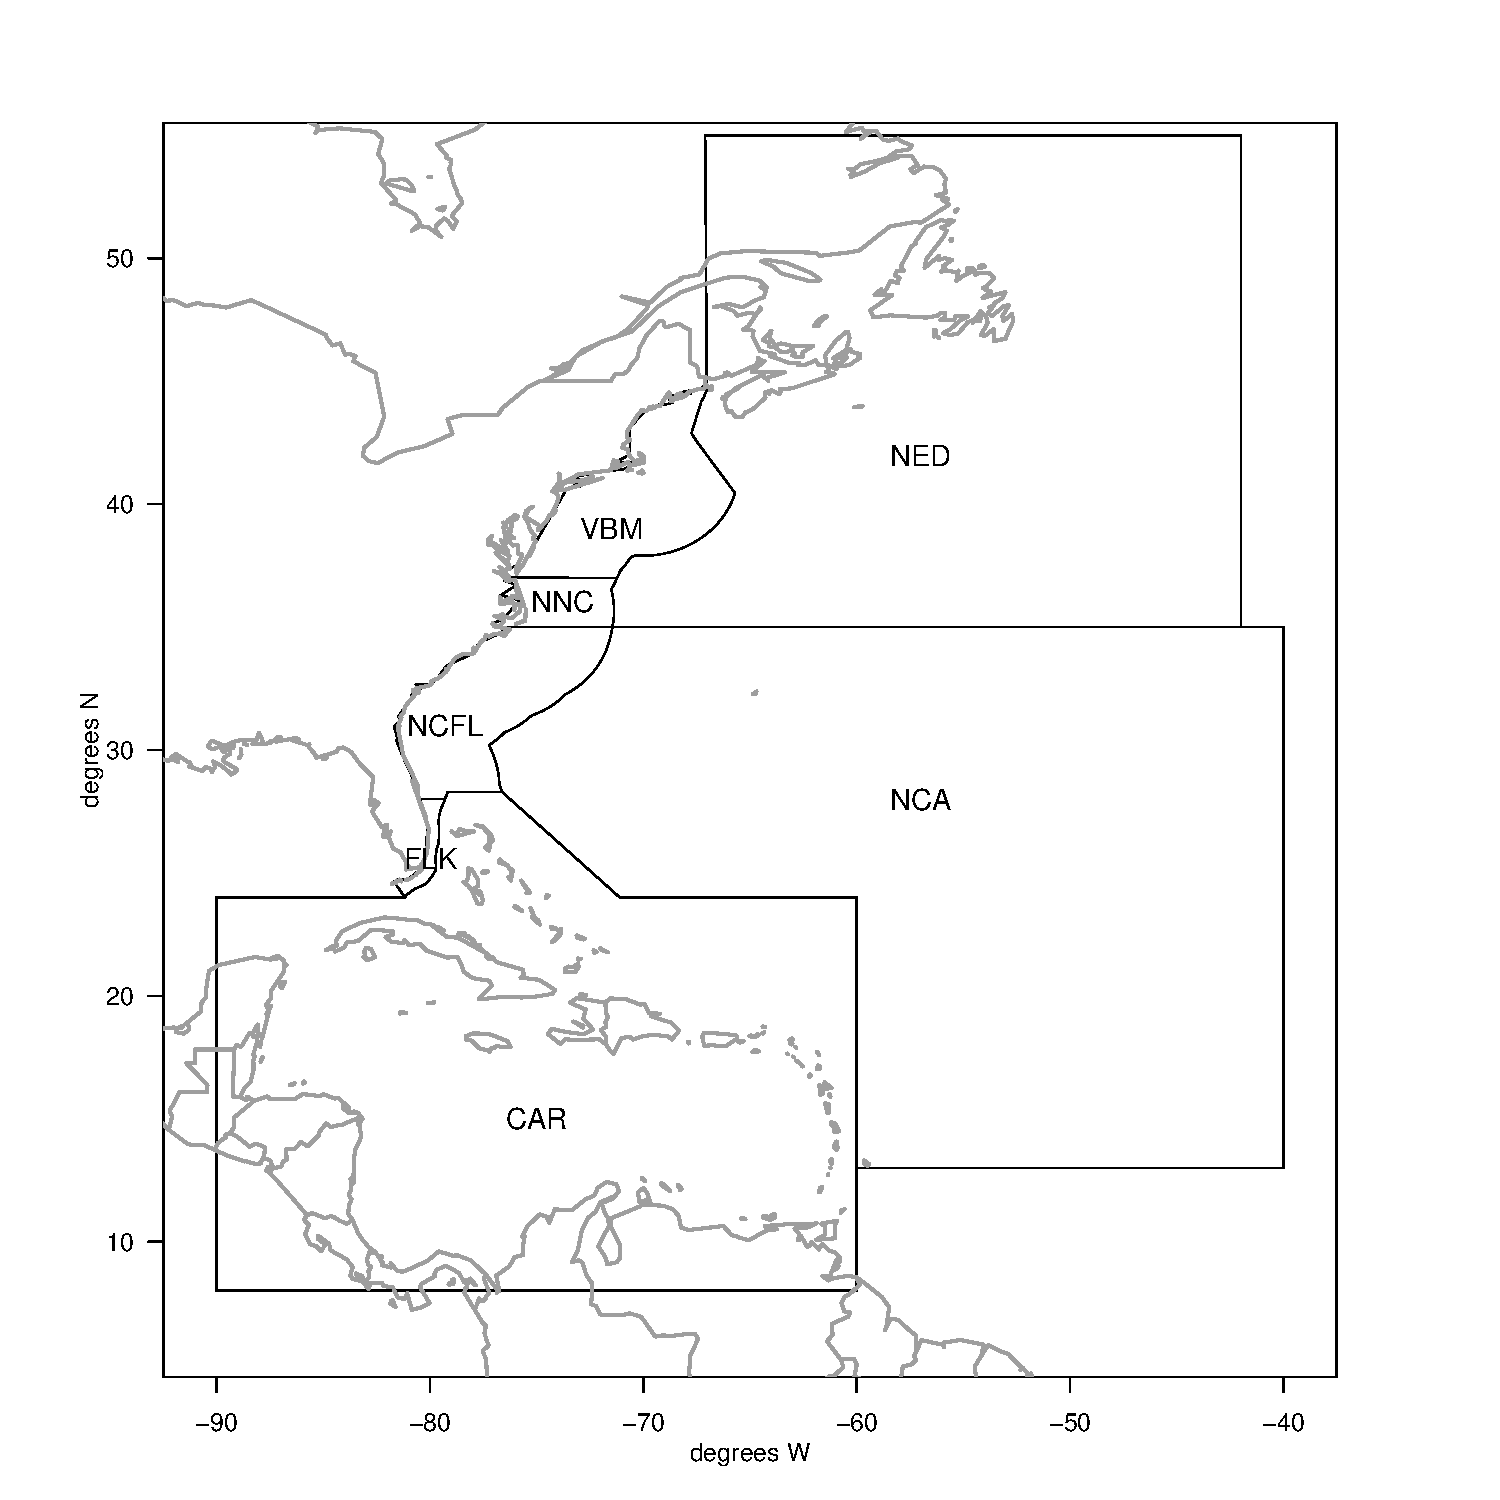
\includegraphics{makeEEZ_files/figure-pdf/unnamed-chunk-10-1.pdf}

\begin{Shaded}
\begin{Highlighting}[]
\CommentTok{\#class(CAR)}

\NormalTok{CAR}\SpecialCharTok{$}\NormalTok{region }\OtherTok{\textless{}{-}} \StringTok{"CAR"}
\NormalTok{FLK}\SpecialCharTok{$}\NormalTok{region }\OtherTok{\textless{}{-}} \StringTok{"FLK"}
\NormalTok{NCFL}\SpecialCharTok{$}\NormalTok{region }\OtherTok{\textless{}{-}} \StringTok{"NCFL"}
\NormalTok{NNC}\SpecialCharTok{$}\NormalTok{region }\OtherTok{\textless{}{-}} \StringTok{"NNC"}
\NormalTok{VBM}\SpecialCharTok{$}\NormalTok{region }\OtherTok{\textless{}{-}} \StringTok{"VBM"}
\NormalTok{NCA}\SpecialCharTok{$}\NormalTok{region }\OtherTok{\textless{}{-}} \StringTok{"NCA"}
\NormalTok{NED}\SpecialCharTok{$}\NormalTok{region }\OtherTok{\textless{}{-}} \StringTok{"NED"}

\NormalTok{zones }\OtherTok{\textless{}{-}} \FunctionTok{rbind}\NormalTok{(FLK, NCFL, NNC, VBM, NED, NCA, CAR)}

\CommentTok{\# plot(zones$X, zones$Y, col = as.numeric(as.factor(zones$region)))}

\CommentTok{\# output the coordinates to a .csv file}
\FunctionTok{write.csv}\NormalTok{(zones, }\AttributeTok{file =} \StringTok{"data/eez/dolphin\_OM\_areas.csv"}\NormalTok{, }\AttributeTok{row.names =} \ConstantTok{FALSE}\NormalTok{)}
\end{Highlighting}
\end{Shaded}





\end{document}
